\chapter{Analysis and Results}

\section{Neural Network}
The first thing to look for is the normality of the errors in the predicted values. If the errors are normally distrubted (and ideally around 0),
then it means that our predictions are sufficiently accurate. We produce a density plot of the errors using the \textit{ggplot2} library in R.

\begin{figure}[h]
    \centering
    \subfloat[\centering Distribution of Errors]{{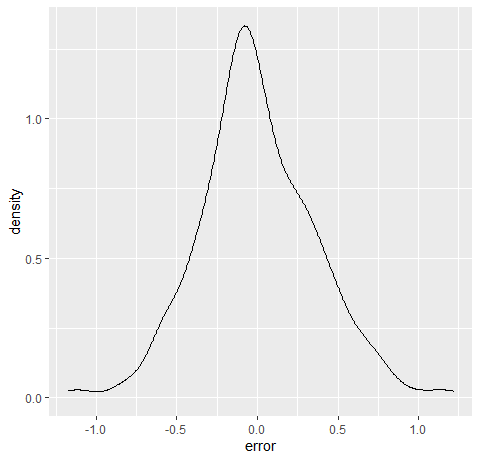
\includegraphics[width=.4\linewidth]{figures/errDist.png} }}
    \qquad
    \subfloat[\centering Q-Q Plot of Errors]{{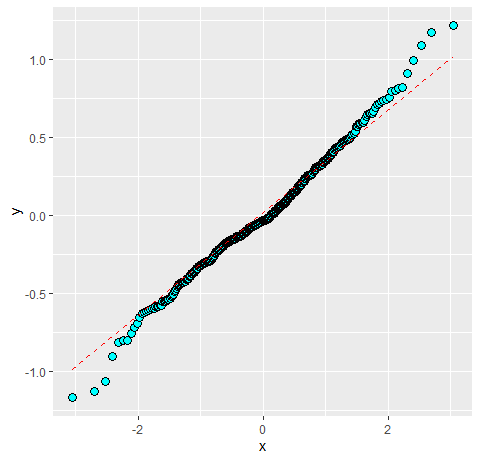
\includegraphics[width=.4\linewidth]{figures/errorqq.png} }}
    \caption{Error distribution with Q-Q plot}
    \label{errDistAndQQ}
\end{figure}

As we can see in this figure, there is a general bell curve, but not quite perfect as we have a bump between -0.5 and -0.75, as well as between 0.125 and 0.5. This 
non-normality is reflected in the Q-Q plot of the error. Measuring accuracy of the results is harder for these value prediction networks is harder than in classification 
problems. This is because we can't construct a prediction matrix. We don't expect the network to predict values down to the exact run, this would require a lot more 
data than is available, and a large amount of experimentation. One metric we can therefore use to see how accurate our model is, is to calculate 
the corrolation between the actual results and the predicted results. Using the inbuilt \textit{cor()} function, we obtain a corrolation value of 
$0.9382$. Given how close this is to 1, which would be perfect corrolation, it is fair to say that this method has done well to predict scores. \\

The issue that one may point out here is that this network has been trained on a full-over dataset, and then been tested on a full-over dataset. But the purpose of this 
investigation has been to look at the scenario in which a full game has been completed. So the method is currently ineffective at doing the task it set out to solve.